% !TeX root = main.tex
\section{Norms and Norm Dependent Linear Regression}

This topic relates to optimization techniques and how to find the maxima or the minima of a curve, how to influence the selection of the parameters. for eg, when reducing the error , there could be many parameters $\vect \theta$ that satisfy an objective function. How do we decide which is the best one, or how do we influence the selection of parameters that satisfy additional criteria such as sparsity? the norms are the kinds of objective functions that force the optimizing methods to select the parameters that satisfy both the objective function and the norm criteria. It will be clearer with the next 4 chapters on optimization techniques. reading additional material is encouraged, since this forms the basis of machine learning.\footnote{\url{https://medium.com/codex/how-norms-drive-the-direction-of-your-optimization-bdbcd619256b}}
\footnote{\url{https://web.stanford.edu/~sidford/courses/20fa_opt_theory/sidford_2020fa_mse213_cs269o_lec8.pdf}}
\footnote{\url{https://utexas.instructure.com/files/43781366/download?download_frd=1}}

Sparsity constraint: we want to force as many dimensions of the parameter vector as possible to zero. 

\subsection{Motivation}

  \begin{itemize}
    \item Different norms and similarity measures play an important role in machine learning and pattern recognition. 
    \item In this chapter we summarize important definitions and facts on norms. 
    \item We consider the problem of linear regression for different norms.
    \item We will briefly look into associated optimization problems.
  \end{itemize}
  
\subsection{Notation in this Chapter}

This chapter follows the notation of numerical linear algebra and optimization (Boyd \& Vandenberghe).\autocite{boyd2004}

\begin{itemize}
  \item $\vect x$, $\vect y$ in the definitions of inner products and norms: generic vectors (not feature vectors / labels).
  \item $\mat A\in\real^{m\times d}$: data (design) matrix -- corresponds to $\mat X$ in the regression part of Chapter \emph{Discriminant Analysis II}.
  \item $\vect x$ in regression problems: unknown parameter vector (optimization variable), not a feature vector -- corresponds to $\vect\theta$.
  \item $\vect b\in\real^m$: target values -- corresponds to $\vect y$.
  \item $\hat{\vect x}$: estimate of the parameter vector, $\vect x_0$: true parameter vector.
  \item $\vect r = \mat A\vect x-\vect b$: residual vector; $\phi$: penalty function (not the LDA feature transform).
\end{itemize}

\subsection{Inner Product}

 \textbf{Definition}

The \textbf{\emph{inner product of vectors}} $\vect x, \vect y\in \real^d$ is defined by \autocite{trefethen1997,golub1996}
    \begin{displaymath}
      \langle\vect x, \vect y\rangle = \vect x^T \vect y = \sum_{i=1}^d x_iy_i \quad .
    \end{displaymath}
Example: The \textbf{\emph{Euclidean norm} ($L_2$-norm)} can be written in terms of an inner product:
    \begin{displaymath}
      \| \vect x \|_2 = \sqrt{\langle \vect x, \vect x \rangle } = 
      \sqrt{ \vect x^T \vect x} = 
      \sqrt{\sum_{i=1}^d x_i^2 }\quad .
    \end{displaymath}
\textbf{Definition}

    The \emph{inner product of matrices} $\mat X, \mat Y\in \real^{m\times n}$ is defined by 
    \begin{displaymath}
       \langle \mat X, \mat Y \rangle = 
       \mbox{tr}(\mat X^T \mat Y) = 
       \sum_{i=1}^m \sum_{j=1}^n x_{i,j} y_{i,j} \quad
    \end{displaymath}
 Example:  The \emph{Frobenius norm} can be written in terms of an inner product:
    \begin{displaymath}
      \| \mat X \|_F = 
      \sqrt{ \langle \mat X, \mat X \rangle } =
      \sqrt{ \mbox{tr}(\mat X^T \mat X)} =
      \sqrt{ \sum_{i=1}^m \sum_{j=1}^n x_{i,j}^2} \quad
    \end{displaymath}

\subsection{Norms}
 \textbf{Definition}

    The function $\lVert\cdot\rVert$ %: \real^d\rightarrow \real$ 
    is called a \textbf{\emph{norm}} if it 
   
    \begin{enumerate}
      \item is \textbf{nonnegative}: $\forall \vect x:~ \lVert\vect x\rVert\geq 0$ 
      \item is \textbf{definite}: $\|\vect x\| =0$ only if $\vect x=\vect 0$ 
      \item is \textbf{homogeneous}: $\| a\vect x\|= |a|\cdot \|\vect x\|$ where $a\in \real$ 
      \item fulfills the \textbf{triangle inequality}:
      \begin{displaymath}
        \forall \vect x, \vect y:~\|\vect x+\vect y\| \leq \|\vect x\|+ \|\vect y\|
      \end{displaymath}
    \end{enumerate}
    \begin{itemize}
      \item The \textbf{$L_0$-norm} of a $d$-dimensional vector denotes the number of    non-zero entries. Despite its name, the $L_0$-norm is not a norm because it is not homogeneous.
      \item The \textbf{$L_p$-norm} ($p \geq 1$) of a $d$-dimensional vector is defined as 
        \begin{displaymath}
          \| \vect x\|_p = \left( \sum_{i=1}^d  |x_i|^p \right)^{\frac{1}{p}}
        \end{displaymath}
    \item \textbf{$L_1$-norm:} sum of absolute values
      \begin{displaymath}
        \| \vect x\|_1 = \sum_{i=1}^d |x_i|
      \end{displaymath}
    
    \item \textbf{$L_2$-norm:} square root of the sum of squared values
      \begin{displaymath}
        \| \vect x\|_2 = \left(\sum_{i=1}^d x_i^2\right)^{\frac{1}{2}}
      \end{displaymath}
    \item \textbf{$L_\infty$-norm:} maximum norm
      \begin{displaymath}
        \| \vect x\|_\infty = 
        \lim_{p\rightarrow \infty} \left( \sum_{i=1}^d  |x_i|^p \right)^{\frac{1}{p}} =
        \max_i \{ |x_i| \ ; \ i=1,2, \dots, d \}
      \end{displaymath}
  \end{itemize}
  \textbf{Definition}
    Let $\mat P$ be a symmetric positive definite matrix.    The \emph{quadratic $L_{\mat P}$-norm} is defined by 
    \begin{displaymath}
      \| \vect x\|_{\mat P} = 
      \sqrt{ \vect x^T \mat P \vect x} = 
      \sqrt{ (\mat P^\frac{1}{2} \vect x)^T \mat P^\frac{1}{2} \vect x} =
      \| \mat P^\frac{1}{2} \vect x\|_2
    \end{displaymath}
  \textbf{Note:} 

  \begin{itemize}
    \item The $L_2$-norm is the same as the quadratic $L_{\mat I}$-norm, where $\mat I$ is the identity matrix.
    \item The \textbf{Mahalanobis distance} between two vectors $\vect x$ and $\vect y$ based on the covariance matrix $\mat \Sigma$ is given by the quadratic $L_{\mat \Sigma^{-1}}$-norm:
      \begin{displaymath}
        \| \vect x - \vect y\|_{\mat \Sigma^{-1}} = 
        \sqrt{ (\vect x - \vect y)^T \mat\Sigma^{-1} (\vect x - \vect y)}
      \end{displaymath}
    \item A norm is a measure for the length of a vector. It can also be used to measure the distance between two vectors $\vect x$ and $\vect y$:
      \begin{displaymath}
        \mbox{dist}(\vect x, \vect y) = \| \vect x - \vect y\|
      \end{displaymath}
  \end{itemize}
  \textbf{Norms of matrices} can be defined by norms of vectors.
  
  \textbf{Definition}
    \small
    Let $\|.\|_p$ and $\|.\|_q$ be norms for vectors in $\real^m$ and $\real^n$. \\
    The \textbf{\emph{operator norm}} of a matrix $\mat X\in \real^{m\times n}$  is defined by
 
    \begin{displaymath}
      \| \mat X\|_{p,q} = \sup\{ \| \mat X \vect u\|_p ; \  \| \vect u\|_q\leq 1 \}
    \end{displaymath}
  Example: If $p=q=2$, i.\,e.\ we use the $L_2$-norm twice, the operator norm of $\mat X$ results in the maximum singular value:
    
    \begin{displaymath}
      \| \mat X\|_{2,2}=   \| \mat X\|_{2} = \sigma_{\max}{(\mat X)}= \sqrt{\lambda_{\max}(\mat X^T\mat X)}
    \end{displaymath}

\subsection{Unit Balls}

The unit ball of a norm is the set of all vectors of norm at most one. Its shape (a diamond for $L_1$, a circle for $L_2$, a square for $L_\infty$ in 2-D) shows which parameter vectors a regularizer with this norm prefers; e.\,g.\ the corners of the $L_1$ ball lie on the axes, which is why the $L_1$-norm favours sparse solutions. 

  \textbf{Definition}
    The set
    \begin{displaymath}
      {\cal B} = \{ \vect x; \|\vect x\| \leq 1\}
    \end{displaymath}
    of all vectors $\vect x$ of length less or equal to one according to the norm $\|.\|$  is called the \textbf{\emph{unit ball}}.
   
 The unit balls for different norms are shown in Fig.~\ref{fig:unitballs}.
  \begin{figure}[htbp]
    \centering
    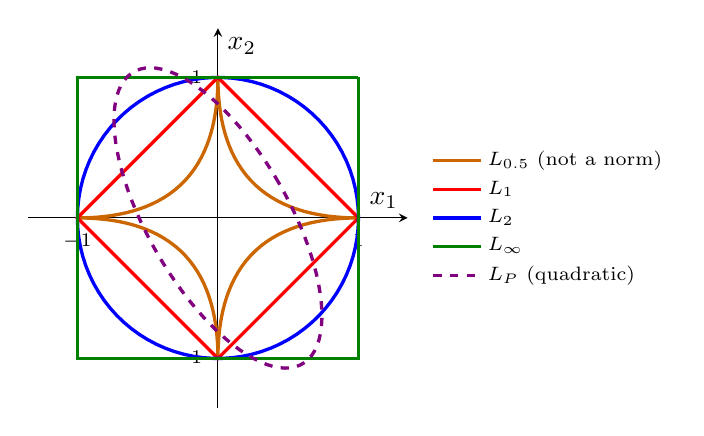
\begin{tikzpicture}
      \begin{axis}[width=6.4cm, height=6.4cm, axis equal image, axis lines=middle, xmin=-1.35, xmax=1.35, ymin=-1.35, ymax=1.35,
          xtick={-1,1}, ytick={-1,1}, tick label style={font=\scriptsize}, xlabel={$x_1$}, ylabel={$x_2$},
          legend style={font=\scriptsize, at={(1.04,0.5)}, anchor=west, draw=none}, legend cell align=left]
        \addplot[orange!80!black, very thick, domain=0:360, samples=181, variable=\t]
          ({sign(cos(\t))*abs(cos(\t))^4}, {sign(sin(\t))*abs(sin(\t))^4});
        \addlegendentry{$L_{0.5}$ (not a norm)}
        \addplot[red, very thick] coordinates {(1,0) (0,1) (-1,0) (0,-1) (1,0)};
        \addlegendentry{$L_1$}
        \addplot[blue, very thick, domain=0:360, samples=91, variable=\t] ({cos(\t)}, {sin(\t)});
        \addlegendentry{$L_2$}
        \addplot[green!50!black, very thick] coordinates {(1,1) (-1,1) (-1,-1) (1,-1) (1,1)};
        \addlegendentry{$L_\infty$}
        \addplot[violet, very thick, dashed, domain=0:360, samples=91, variable=\t]
          ({0.5*cos(\t)*cos(30)-1.2*sin(\t)*sin(30)}, {0.5*cos(\t)*sin(30)+1.2*sin(\t)*cos(30)});
        \addlegendentry{$L_{\mat P}$ (quadratic)}
      \end{axis}
    \end{tikzpicture}
    \caption{Boundaries of the unit balls $\{\vect x;\ \|\vect x\|\le1\}$ in $\real^2$: $L_1$ (diamond), $L_2$ (circle), $L_\infty$ (square), and a quadratic norm $L_{\mat P}$ (ellipse whose axes are the eigenvectors of $\mat P$, with semi-axis lengths $1/\sqrt{\lambda_i(\mat P)}$). For $p<1$ the ``ball'' $\{\vect x;\ (\sum_i|x_i|^p)^{1/p}\le1\}$ (shown for $p=0.5$) is not convex, i.\,e.\ the triangle inequality fails and $L_p$ is not a norm. For $p\ge1$ the balls are nested: $L_1\subset L_2\subset L_\infty$.}
    \label{fig:unitballs}
  \end{figure}

 \textbf{Exam notes:} It is important to know the difference and to understand what are unit balls.Remember that the $L_{0.5}$- and the $L_0$-norm are not norms

\subsection{Norm Dependent Linear Regression}

  In pattern recognition and pattern analysis (as in many other fields) one of the most important norm dependent linear regression problems is:

  \begin{displaymath}
   \mbox{minimize}\quad \| \mat A \vect x -\vect b\|
  \end{displaymath}
  or alternatively
  \begin{displaymath}
   \hat{\vect x} = \argmin_{\vect x} \| \mat A \vect x -\vect b\|
  \end{displaymath}
 \begin{itemize}
    \item Different norms will lead to different results. 
    \item The estimation error $\epsilon\in \real$ is defined by $\epsilon= \|\vect x_0-\hat{\vect x}\|$, where $\vect x_0$ denotes the correct (true) value. 
    \item The \textbf{residual} $\vect r= (r_1, r_2, \dots, r_m)^T$ is defined by $\vect r= \mat A \vect x -\vect b$. \\
    \item If $\vect b$ is in the range of $\mat A$, the residual of the optimal solution is the zero vector (for any norm).
  \end{itemize}
  
\subsubsection{Least-Squares Linear Regression}

  \textbf{Minimization of the residual using the $L_2$-norm:}
  \begin{eqnarray*}
    \hat{\vect x} &=& \argmin_{\vect x} \| \mat A \vect x -\vect b\|_2 \\
                 &=& \argmin_{\vect x} \sum_{i=1}^m r_i^2 \\
                 &=& \argmin_{\vect x} \ (\mat A \vect x -\vect b)^T (\mat A \vect x -\vect b) \\
                 &=& \argmin_{\vect x} \ \big( \vect x^T \mat A^T \mat A\vect x - \vect x^T\mat A^T \vect b - \vect b^T \mat A\vect x + \vect b^T \vect b \big) \\
                 &=& \argmin_{\vect x} \ \big( \vect x^T \mat A^T \mat A\vect x - 2 \vect b^T \mat A\vect x + \vect b^T \vect b \big) \\
  \end{eqnarray*}
  The \textbf{partial derivatives} are:
  \begin{displaymath}
    \frac{\partial}{\partial \vect x} \ \left( \vect x^T \mat A^T \mat A\vect x - 2 \vect b^T \mat A\vect x + \vect b^T \vect b \right)
    = 2 \mat A^T \mat A \vect x - 2 \mat A^T \vect b = \vect{0}
  \end{displaymath}
  Using the partial derivatives we get a \textbf{closed form solution} for the $L_2$-norm: 
  \begin{displaymath}
    \hat{\vect x} = (\mat A^T \mat A)^{-1}\mat A^T \vect b
  \end{displaymath}
  if the columns of $\mat A$ are linearly independent.
 
\subsubsection{Chebyshev Linear Regression}

  \textbf{Minimization of the residual using the $L_\infty$-norm:}
  \begin{displaymath}
    \mbox{minimize}\quad \Bigg\{ \| \mat A \vect x -\vect b\|_\infty = \max\ \{ |r_1|, |r_2|, \dots, |r_m|\} \Bigg\}
  \end{displaymath}
  This optimization problem can be rewritten in terms of a LP-problem:
  \begin{eqnarray*}
    \begin{array}{lcl}
     \mbox{minimize}& & t\\
     \mbox{subject to} & &   - t\cdot \vect 1 \preceq \mat A \vect x - \vect b \preceq t\cdot \vect 1
    \end{array}
  \end{eqnarray*}
  over $\vect x$ and an auxiliary bound $t\in \real$ (i.\,e.\ $|r_i|\le t$ for all residual components), where $\vect 1 \in \{1\}^m$ is the all-ones vector and $\preceq$ denotes componentwise inequality.


  
\subsubsection{Sum of Absolute Residuals}
\textbf{Minimization of the residual using the $L_1$-norm:}
  \begin{displaymath}
    \mbox{minimize}\quad \Bigg\{ \| \mat A \vect x -\vect b\|_1 = \sum_{i=1}^m  |r_i| \Bigg\}
  \end{displaymath}
  This optimization problem can be rewritten in terms of a LP-problem:
  \begin{eqnarray*}
    \begin{array}{lcl}
      \mbox{minimize}   & & \vect 1^T \vect t \\
      \mbox{subject to} & & - \vect t \preceq  \mat A \vect x -\vect b\preceq \vect  t
    \end{array}
  \end{eqnarray*}
  over $\vect x$ and auxiliary bounds $\vect t\in \real^m$ (i.\,e.\ $|r_i|\le t_i$), and $\vect 1 \in \{1\}^m$.
 
\subsubsection{Ridge Regression and Unit Balls}
\textbf{Ridge regression} is defined via the optimization problem
  \begin{displaymath}
    \mbox{minimize} \quad \|\mat A\vect x -\vect b\|_2^2+\lambda \cdot\|\vect x\|_2^2
  \end{displaymath}
 
\subsubsection{Lasso and Unit Balls}
  The \textbf{lasso} (Tibshirani 1996) is defined via the optimization problem
  \begin{displaymath}
    \mbox{minimize} \quad \|\mat A\vect x -\vect b\|_2^2+\lambda \cdot\|\vect x\|_1
  \end{displaymath}
  Figure~\ref{fig:ridge_lasso} compares the geometry of ridge regression and the lasso: the corners of the $L_1$ ball make exactly-zero coefficients likely.

  \begin{figure}[htbp]
    \centering
    \begin{tikzpicture}
      \begin{groupplot}[group style={group size=2 by 1, horizontal sep=1.2cm}, width=6.2cm, height=6.2cm,
          axis equal image, axis lines=middle, xmin=-1.4, xmax=3.9, ymin=-1.4, ymax=3.6, xtick={-1,1,2,3}, ytick={-1,1,2,3},
          tick label style={font=\scriptsize}, title style={font=\small}, xlabel={$x_1$}, ylabel={$x_2$}]
        \nextgroupplot[title={Ridge: $\|\vect x\|_2\le t$}]
\addplot[blue, very thick, fill=blue!12, domain=0:360, samples=121, variable=\t] ({cos(\t)}, {sin(\t)});
\addplot[gray, thin, domain=0:360, samples=121, variable=\t] ({1.4+0.6325*cos(\t)*0.8660-0.2582*sin(\t)*-0.5000}, {1.2+0.6325*cos(\t)*-0.5000+0.2582*sin(\t)*0.8660});
\addplot[gray, thin, domain=0:360, samples=121, variable=\t] ({1.4+1.2247*cos(\t)*0.8660-0.5000*sin(\t)*-0.5000}, {1.2+1.2247*cos(\t)*-0.5000+0.5000*sin(\t)*0.8660});
\addplot[black, thick, domain=0:360, samples=121, variable=\t] ({1.4+1.8940*cos(\t)*0.8660-0.7730*sin(\t)*-0.5000}, {1.2+1.8940*cos(\t)*-0.5000+0.7730*sin(\t)*0.8660});
\addplot[only marks, mark=*, mark size=1.6pt, black] coordinates {(1.4,1.2)} node[above right, font=\scriptsize] {$\hat{\vect x}_{\text{LS}}$};
\addplot[only marks, mark=*, mark size=2pt, red] coordinates {(0.593,0.805)} node[left, font=\scriptsize, xshift=-2pt, fill=white, inner sep=1pt] {$(0.59,\,0.80)$};
\nextgroupplot[title={Lasso: $\|\vect x\|_1\le t$}]
\addplot[red, very thick, fill=red!12] coordinates {(1,0) (0,1) (-1,0) (0,-1) (1,0)};
\addplot[gray, thin, domain=0:360, samples=121, variable=\t] ({1.4+0.6325*cos(\t)*0.8660-0.2582*sin(\t)*-0.5000}, {1.2+0.6325*cos(\t)*-0.5000+0.2582*sin(\t)*0.8660});
\addplot[gray, thin, domain=0:360, samples=121, variable=\t] ({1.4+1.2247*cos(\t)*0.8660-0.5000*sin(\t)*-0.5000}, {1.2+1.2247*cos(\t)*-0.5000+0.5000*sin(\t)*0.8660});
\addplot[gray, thin, domain=0:360, samples=121, variable=\t] ({1.4+1.8974*cos(\t)*0.8660-0.7746*sin(\t)*-0.5000}, {1.2+1.8974*cos(\t)*-0.5000+0.7746*sin(\t)*0.8660});
\addplot[black, thick, domain=0:360, samples=121, variable=\t] ({1.4+2.4110*cos(\t)*0.8660-0.9840*sin(\t)*-0.5000}, {1.2+2.4110*cos(\t)*-0.5000+0.9840*sin(\t)*0.8660});
\addplot[only marks, mark=*, mark size=1.6pt, black] coordinates {(1.4,1.2)} node[above right, font=\scriptsize] {$\hat{\vect x}_{\text{LS}}$};
\addplot[only marks, mark=*, mark size=2pt, red] coordinates {(0,1)} node[left, font=\scriptsize, xshift=-2pt, fill=white, inner sep=1pt] {$(0,\,1)$};
      \end{groupplot}
    \end{tikzpicture}
    \caption{Why the lasso gives sparse solutions (constrained form with $t=1$; the penalized forms above are equivalent for a suitable $\lambda$). Gray: contour lines of the least-squares cost $\|\mat A\vect x-\vect b\|_2^2$, which are ellipses around the unregularized solution $\hat{\vect x}_{\text{LS}}$. The constrained solution (red dot) is where the smallest contour touches the unit ball (black contour). The round $L_2$ ball is touched at a generic point with both components non-zero. The $L_1$ ball has corners on the axes, and the contour typically touches it at a corner, so $x_1=0$ exactly.}
    \label{fig:ridge_lasso}
  \end{figure}

\subsubsection{Compressed Sensing}\autocite{candes2008,boyd2004}
\begin{itemize}
    \item In the previous chapter we motivated regularized linear regression. 
    \item Assume we have fewer measurements than required to estimate the parameter vector $\vect x$. 
    \item Solution of the underdetermined case required. 
    \item We call a vector $s$-sparse if its support, i.\,e.\ the number of non-zero entries, is less than or equal to $s$ ($S$ is reserved for the training set).  
    \item Under suitable conditions on the sparsity $s$ and on the measurement matrix $\mat A$ (e.\,g.\ a restricted isometry or null-space property), an $s$-sparse vector $\vect x$ is recovered \emph{exactly} from noiseless measurements by solving the convex optimization problem (it can be rewritten as a linear program):
      \begin{eqnarray*}
        \mbox{minimize}   & &\quad \|\vect x\|_1\\
        \mbox{subject to} & & \quad \mat A\vect x =\vect b.
      \end{eqnarray*}
      For noisy measurements the constraint is relaxed, e.\,g.\ to $\|\mat A\vect x-\vect b\|_2\le\varepsilon$, or a penalized form (lasso) is used.
  \end{itemize}

\newpage
\subsection{Convex and Non-Convex Penalty Functions}

  Motivated by the discussion of different norms, we now introduce and study \textbf{penalty functions}. A penalty function $\phi$ assigns a cost to each residual; norms are special cases (e.\,g.\ $\phi(r)=|r|$ or $r^2$), and norms can also be used as regularizers on the parameters (e.\,g.\ $\lambda\|\vect x\|_1$). Both convex and non-convex objectives can be optimized, but convexity is very useful: every local minimum of a convex function is global. Non-convex problems may have several local minima, so finding or certifying the global optimum is harder (see the optimization chapters).\\[0.3cm]
  
  \textbf{Definition}\\
The \emph{penalty function approximation problem} is defined as follows:
    \begin{eqnarray*}
      \mbox{minimize}   & &\sum_{i=1}^m \phi(r_i) \\
      \mbox{subject to} & & \vect r= (r_1, r_2, \dots, r_m)^T = \mat A\vect x -\vect b,
    \end{eqnarray*}
    where $\phi:\real \rightarrow \real$ is the penalty function for the components of the \\
    residual vector.
    
  \textbf{Note:} 
  \begin{itemize}
    \item The penalty function $\phi$ assigns \textbf{costs} to residuals. 
    \item If $\phi$ is a convex function, the penalty function approximation problem is a convex optimization problem.
  \end{itemize}
  Penalty functions of the $L_1$-,  $L_2$-norms:
  \begin{displaymath}
    \phi_{L_1}(r) = |r|;  \qquad \qquad \qquad \qquad \qquad \phi_{L_2}(r) = r^2
  \end{displaymath}
  \begin{itemize}
    \item In $L_1$ small deviations are weighted higher than using $L_2$.
    \item In $L_1$ large deviations are weighted lower than using $L_2$.
  \end{itemize}
 \textbf{Log barrier function} with parameter $a>0$
  \begin{displaymath}
    \phi_\mathsf{barrier}(r) = 
      \left\{
        \begin{array}{cl}
          -a^2\log \left(1-\left( \frac{r}{a}\right)^2 \right),  & \quad \mbox{if} \quad |r| < a\\
          \infty,                                                & \quad \mbox{otherwise}
        \end{array}
      \right.
  \end{displaymath}   
  \textbf{Dead zone linear penalty function} with parameter $a>0$
  \begin{displaymath}
    \phi_\mathsf{dz}(r) = 
      \left\{
        \begin{array}{cl}
          0,     & \quad \mbox{if} \quad |r| \leq a\\
          |r|-a, & \quad \mbox{otherwise}
        \end{array}
      \right.
  \end{displaymath}
  \textbf{Large error penalty function} with parameter $a>0$
  \begin{displaymath}
    \phi_\mathsf{e}(r) = 
      \left\{
        \begin{array}{cl}
          r^2, & \quad \mbox{if} \quad |r| \leq a \\
          a^2, & \quad \mbox{otherwise}
        \end{array}
      \right.
  \end{displaymath}
  \textbf{Huber function} with parameter $a>0$
  \begin{displaymath}
    \phi_\mathsf{Huber}(r) = 
      \left\{
        \begin{array}{cl}
          r^2,            & \quad \mbox{if} \quad |r| \leq a \\
          a\cdot(2|r|-a), & \quad \mbox{otherwise}
        \end{array}
      \right.
  \end{displaymath}
  
\subsection{Lessons Learned}
  \begin{itemize}
    \item We have considered vector and matrix norms in more detail. 
    \item Important vector norms: $L_1$, $L_2$, $L_\infty$, and $L_{\mat P}$. 
    \item Unit balls 
    \item Linear regression for different norms: range from closed form solution to LP-problem.
    \item Regularized linear regression: range from closed form solution through QP-problem up to combinatorial optimization. 
    \item We need to know the basics of algorithms for unconstrained and constrained optimization as well as convex optimization.
  \end{itemize}

\subsection{Comprehensive Questions}
  \begin{itemize}
    \item What is the difference between the $L_p$- (p $\ge$ 1) and the $L_{\mat P}$-norm? 
    \item How do the unit balls look like for $L_{\infty}$-, $L_4$-, $L_2$-, $L_1$- and $L_0$-norm? 
    \item What is the benefit of using the $L_1$- over the $L_2$-norm for sparse, underdetermined problems? 
    \item What specific property of penalty functions is of special interest and why do we need different penalty functions at all? 
  \end{itemize}

\newpage
\section{Rosenblatt's Perceptron (1957)}\autocite{hastie2009,ripley1996,rosenblatt1958}

\subsection{Motivation}

The perceptron, developed by Frank Rosenblatt in 1957, is considered the first model of an artificial neural network. Its goal is to compute a linear decision boundary between two classes. We therefore assume that the classes are \textbf{linearly separable}, i.\,e.\ that there exists a hyperplane which classifies every training example correctly. The learning task is then to compute such a linear separating hyperplane by minimizing the distance of the misclassified feature vectors to the decision boundary.

\subsection{Objective Function}

  Assume the following:
  \begin{itemize}
    \item True class labels are $y_i\in\{-1,+1\}$.
    \item The decision boundary is a linear function with prediction
      \begin{displaymath}
        \hat y = \sign(\vect \alpha^T\vect x + \alpha_0).
      \end{displaymath}
    \item Parameters $\alpha_0$ and $\vect \alpha$ are chosen according to the optimization problem 
      \begin{center}
        $\displaystyle \mbox{minimize} \quad \bigg\{ D(\alpha_0, \vect \alpha)= -\sum_{i\in {\cal M}} y_i \cdot (\vect \alpha^T\vect x_i + \alpha_0) \bigg\}$
      \end{center}
      where $\cal M$ is the set of \textbf{indices} of misclassified samples.
     \item The elements of the sum in the objective function depend on the set $\cal M$.          
    \item In each iteration step the cardinality of $\cal M$ might change.          
    \item The cardinality of $\cal M$ is a discrete variable.
    \item \textbf{Competing variables:} continuous parameters of linear decision boundary and the discrete cardinality of $\cal M$.
  \end{itemize}
 
\subsection{Minimization of Objective Function}

  Remember the objective function $D(\alpha_0, \vect \alpha)$:
  \begin{displaymath}
    \mbox{minimize} \quad \quad D(\alpha_0, \vect \alpha)= -\sum_{i\in {\cal M}} y_i \cdot (\vect \alpha^T\vect x_i + \alpha_0)
  \end{displaymath}
 
  The gradient of the objective function is:          
  \begin{eqnarray*}
    \frac{\partial}{\partial \alpha_0} \ D(\alpha_0, \vect \alpha)&=&  -\sum_{i\in {\cal M}} y_i \\          
    \frac{\partial}{\partial \vect\alpha} \ D(\alpha_0, \vect \alpha)&=& -\sum_{i\in {\cal M}} y_i\cdot  \vect x_i \\
  \end{eqnarray*}
  We want to take an update step right after having visited each misclassified observation.
  The update rule in the $(k+1)$-st iteration step is:

  \begin{displaymath}
    \begin{pmatrix}\alpha_0^{(k+1)}\\ \vect \alpha^{(k+1)}\end{pmatrix} =            \begin{pmatrix}\alpha_0^{(k)}\\ \vect \alpha^{(k)}\end{pmatrix} + \eta \begin{pmatrix}y_i\\ y_i\cdot \vect x_i\end{pmatrix}
  \end{displaymath} 
  Here $\eta>0$ is the learning rate (step size; the same symbol is used in the MLP chapter). With the zero initialization below it can be set to $1$ without loss of generality, since it only scales $(\alpha_0,\vect\alpha)$. The parameters are stacked as $(\alpha_0;\vect\alpha)$ here, while the regression part of Chapter \emph{Discriminant Analysis} stacks $\vect\theta=(\vect\alpha;\alpha_0)$; the order does not matter.
 
  \begin{algorithmic}
    \STATE\textbf{Input:} training data: $S = \{(\vect x_i,y_i)\}_{i=1}^m$ with $y_i\in\{-1,+1\}$.
    \STATE initialize  $k=0$, $\alpha^{(0)}_0=0$ and $\vect \alpha^{(0)}=  \vect 0$
    \Repeat
      \STATE select pair $(\vect x_i, y_i)$ from training set.
      \If{$y_i\cdot (\vect x_i^T \vect\alpha^{(k)} + \alpha_0^{(k)})\leq 0$}
        \STATE
        \STATE $\displaystyle\begin{pmatrix}\alpha_0^{(k+1)}\\ \vect \alpha^{(k+1)}\end{pmatrix} =  \begin{pmatrix}\alpha_0^{(k)}\\ \vect \alpha^{(k)}\end{pmatrix} +  \begin{pmatrix}y_i\\ y_i\cdot \vect x_i\end{pmatrix}$
        \STATE
        \STATE $k\leftarrow k+1$
      \EndIf

    \Until{$y_i\cdot (\vect x_i^T \vect\alpha^{(k)} + \alpha_0^{(k)})> 0 \quad \mbox {for all} \quad i$}
    \STATE \structure{Output:} $\alpha_0^{(k)}$ and $\vect \alpha^{(k)}$
  \end{algorithmic}

Figure~\ref{fig:perceptron_updates} shows the algorithm on a small example.

  \begin{figure}[htbp]
    \centering
    \begin{tikzpicture}
      \begin{groupplot}[group style={group size=2 by 2, horizontal sep=0.9cm, vertical sep=1.1cm}, width=5.6cm, height=5.6cm,
          axis equal image, xmin=-2.8, xmax=2.8, ymin=-2.8, ymax=2.8, xtick={-2,0,2}, ytick={-2,0,2},
          tick label style={font=\scriptsize}, title style={font=\small}]
        \nextgroupplot[title={after update $k=1$}]
\addplot[only marks, mark=*, mark size=1.3pt, red!70] coordinates {(0.51,0.30) (1.90,0.80) (0.53,0.49) (-0.06,0.55) (1.04,1.35) (1.09,0.71) (0.00,1.75) (-0.25,1.06) (0.70,-0.13) (0.51,-0.00) (1.13,0.33) (1.79,-0.70) (0.90,-0.14) (1.37,-0.87)};
\addplot[only marks, mark=square*, mark size=1.2pt, blue!70] coordinates {(-0.81,-0.37) (-1.49,0.09) (-0.49,0.10) (-0.02,-1.09) (-1.08,-0.62) (-0.15,0.01) (-1.03,-0.86) (-1.08,-0.85) (-0.74,-0.58) (0.63,-0.80) (-0.77,-0.22) (-1.17,-0.72) (-0.59,-0.04) (-1.39,0.32) (-0.81,-0.40)};
\addplot[only marks, mark=o, mark size=3pt, thick, orange!90!black] coordinates {(-0.81,-0.37) (-1.49,0.09) (-0.49,0.10) (-0.02,-1.09) (-1.08,-0.62) (-0.15,0.01) (-1.03,-0.86) (-1.08,-0.85) (-0.74,-0.58) (0.63,-0.80) (-0.77,-0.22) (-1.17,-0.72) (-0.59,-0.04) (-1.39,0.32) (-0.81,-0.40)};
\addplot[only marks, mark=diamond, mark size=4pt, very thick, black] coordinates {(0.51,-0.00)};
\addplot[black, very thick] coordinates {(-1.993,-2.800) (-1.958,2.800)};
\draw[-{Stealth}, thick, green!50!black] (axis cs:-1.976,0.000) -- (axis cs:-1.176,-0.005) node[above, font=\scriptsize] {$\vect\alpha^{(k)}$};
        \nextgroupplot[title={after update $k=3$}]
\addplot[only marks, mark=*, mark size=1.3pt, red!70] coordinates {(0.51,0.30) (1.90,0.80) (0.53,0.49) (-0.06,0.55) (1.04,1.35) (1.09,0.71) (0.00,1.75) (-0.25,1.06) (0.70,-0.13) (0.51,-0.00) (1.13,0.33) (1.79,-0.70) (0.90,-0.14) (1.37,-0.87)};
\addplot[only marks, mark=square*, mark size=1.2pt, blue!70] coordinates {(-0.81,-0.37) (-1.49,0.09) (-0.49,0.10) (-0.02,-1.09) (-1.08,-0.62) (-0.15,0.01) (-1.03,-0.86) (-1.08,-0.85) (-0.74,-0.58) (0.63,-0.80) (-0.77,-0.22) (-1.17,-0.72) (-0.59,-0.04) (-1.39,0.32) (-0.81,-0.40)};
\addplot[only marks, mark=o, mark size=3pt, thick, orange!90!black] coordinates {(-0.81,-0.37) (-0.49,0.10) (-0.02,-1.09) (-0.15,0.01) (-0.74,-0.58) (0.63,-0.80) (-0.77,-0.22) (-0.59,-0.04) (-0.81,-0.40)};
\addplot[only marks, mark=diamond, mark size=4pt, very thick, black] coordinates {(1.37,-0.87)};
\addplot[black, very thick] coordinates {(-0.967,-2.800) (-0.650,2.800)};
\draw[-{Stealth}, thick, green!50!black] (axis cs:-0.808,0.000) -- (axis cs:-0.010,-0.045) node[above, font=\scriptsize] {$\vect\alpha^{(k)}$};
        \nextgroupplot[title={after update $k=6$}]
\addplot[only marks, mark=*, mark size=1.3pt, red!70] coordinates {(0.51,0.30) (1.90,0.80) (0.53,0.49) (-0.06,0.55) (1.04,1.35) (1.09,0.71) (0.00,1.75) (-0.25,1.06) (0.70,-0.13) (0.51,-0.00) (1.13,0.33) (1.79,-0.70) (0.90,-0.14) (1.37,-0.87)};
\addplot[only marks, mark=square*, mark size=1.2pt, blue!70] coordinates {(-0.81,-0.37) (-1.49,0.09) (-0.49,0.10) (-0.02,-1.09) (-1.08,-0.62) (-0.15,0.01) (-1.03,-0.86) (-1.08,-0.85) (-0.74,-0.58) (0.63,-0.80) (-0.77,-0.22) (-1.17,-0.72) (-0.59,-0.04) (-1.39,0.32) (-0.81,-0.40)};
\addplot[only marks, mark=o, mark size=3pt, thick, orange!90!black] coordinates {(-0.25,1.06) (0.63,-0.80)};
\addplot[only marks, mark=diamond, mark size=4pt, very thick, black] coordinates {(1.37,-0.87)};
\addplot[black, very thick] coordinates {(-0.457,2.800) (0.457,-2.800)};
\draw[-{Stealth}, thick, green!50!black] (axis cs:0.000,0.000) -- (axis cs:0.790,0.129) node[above, font=\scriptsize] {$\vect\alpha^{(k)}$};
        \nextgroupplot[title={after update $k=11$ (converged)}]
\addplot[only marks, mark=*, mark size=1.3pt, red!70] coordinates {(0.51,0.30) (1.90,0.80) (0.53,0.49) (-0.06,0.55) (1.04,1.35) (1.09,0.71) (0.00,1.75) (-0.25,1.06) (0.70,-0.13) (0.51,-0.00) (1.13,0.33) (1.79,-0.70) (0.90,-0.14) (1.37,-0.87)};
\addplot[only marks, mark=square*, mark size=1.2pt, blue!70] coordinates {(-0.81,-0.37) (-1.49,0.09) (-0.49,0.10) (-0.02,-1.09) (-1.08,-0.62) (-0.15,0.01) (-1.03,-0.86) (-1.08,-0.85) (-0.74,-0.58) (0.63,-0.80) (-0.77,-0.22) (-1.17,-0.72) (-0.59,-0.04) (-1.39,0.32) (-0.81,-0.40)};
\addplot[only marks, mark=diamond, mark size=4pt, very thick, black] coordinates {(0.63,-0.80)};
\addplot[black, very thick] coordinates {(-1.936,2.800) (2.674,-2.800)};
\draw[-{Stealth}, thick, green!50!black] (axis cs:0.369,0.000) -- (axis cs:0.987,0.508) node[above, font=\scriptsize] {$\vect\alpha^{(k)}$};
      \end{groupplot}
    \end{tikzpicture}
    \caption{Perceptron learning on a linearly separable toy set (red circles: $y=+1$, blue squares: $y=-1$), zero initialization, learning rate $1$. Each update adds $y_i(1,\vect x_i^T)^T$ of the currently visited misclassified sample (black diamond) to $(\alpha_0,\vect\alpha^T)^T$, which rotates and shifts the boundary $\vect\alpha^T\vect x+\alpha_0=0$ (black; the green arrow is the normal $\vect\alpha^{(k)}$ pointing to the $\hat y=+1$ side). Orange rings mark the samples that are still misclassified. Here the algorithm stops after $11$ updates, well below the Novikoff bound (Fig.~\ref{fig:perceptron_margin}).}
    \label{fig:perceptron_updates}
  \end{figure}

\subsection{Remarks on Perceptron Learning}

  \begin{itemize}
    \item The update rule is extremely simple. \\[.3cm]
    \item Nothing happens if we classify all $\vect x_i$ correctly using the given linear decision boundary. 
    \item The parameter $\vect \alpha$ of the decision boundary is a linear combination of feature vectors. 
    \item The decision boundary thus is:
    \begin{displaymath}
       f(\vect x) = \left (\sum_{i\in \cal E} y_i\cdot \vect x_i \right)^T \vect x + \sum_{i\in \cal E} y_i \quad 
                 = \quad \sum_{i\in \cal E} y_i\cdot \langle \vect x_i, \vect x\rangle + \sum_{i\in \cal E} y_i 
    \end{displaymath}
    with $\hat y=\sign(f(\vect x))$, where $\cal E$ is the list of indices that required an update (indices may appear more than once); this assumes zero initialization and $\eta=1$. 
    \item The final linear decision boundary depends on the initialization, \\
      i.\,e.\ $\alpha_0^{(0)}$ and $\vect \alpha^{(0)}$. 
    \item The number of iterations can be rather large. 
    \item If data are not linearly separable, the proposed learning algorithm will not converge. The algorithm will end up in hard to detect cycles.
  \end{itemize}

\subsection{Convergence of Learning Algorithm}

The derivation is not important for the exam. It is important to understand that, for linearly separable data, there is an \emph{upper bound} on the number of updates the perceptron makes before it classifies all training samples correctly. The bound depends on the margin $\rho$, the data radius $R$ and the offset $\alpha_0^*$ of the separating hyperplane, not explicitly on the feature dimension. 

 \textbf{Convergence Theorem of Rosenblatt and Novikoff}\\
    Assume that for all $i=1,2, \dots, m$
    \begin{displaymath}
      y_i(\vect x_i^T\vect \alpha^* +\alpha^*_0)\geq \rho
    \end{displaymath}
    for some $(\alpha_0^*,\vect\alpha^*)$ with $\rho>0$ and $\|\vect \alpha^*\|_2=1$ (i.\,e.\ the data are linearly separable with margin $\rho$).
    Let $R= \max_i \|\vect x_i\|_2$. \\
    
Then the perceptron learning algorithm with zero initialization makes at most $k$ updates (and then separates the training data), where
    \begin{displaymath}
      k \leq \frac{(\alpha_0^{*2}+1)(1+R^2)}{\rho^2}.
    \end{displaymath}
    The quantities $\rho$ and $R$ are illustrated in Fig.~\ref{fig:perceptron_margin}.

  \begin{figure}[htbp]
    \centering
    \begin{tikzpicture}
      \begin{axis}[width=7.2cm, height=7.2cm, axis equal image, xmin=-2.9, xmax=2.9, ymin=-2.9, ymax=2.9,
          xtick={-2,0,2}, ytick={-2,0,2}, tick label style={font=\scriptsize}, clip=false]
        \fill[gray!12] (axis cs:-2.320,2.800) -- (axis cs:2.800,-2.320) -- (axis cs:2.659,-2.800) -- (axis cs:-2.800,2.659) -- cycle;
        \draw[gray!60, dashed] (axis cs:0,0) circle [radius=2.058];
        \addplot[only marks, mark=*, mark size=1.3pt, red!70] coordinates {(0.51,0.30) (1.90,0.80) (0.53,0.49) (-0.06,0.55) (1.04,1.35) (1.09,0.71) (0.00,1.75) (-0.25,1.06) (0.70,-0.13) (0.51,-0.00) (1.13,0.33) (1.79,-0.70) (0.90,-0.14) (1.37,-0.87)};
        \addplot[only marks, mark=square*, mark size=1.2pt, blue!70] coordinates {(-0.81,-0.37) (-1.49,0.09) (-0.49,0.10) (-0.02,-1.09) (-1.08,-0.62) (-0.15,0.01) (-1.03,-0.86) (-1.08,-0.85) (-0.74,-0.58) (0.63,-0.80) (-0.77,-0.22) (-1.17,-0.72) (-0.59,-0.04) (-1.39,0.32) (-0.81,-0.40)};
        \addplot[black, very thick] coordinates {(-2.630,2.800) (2.800,-2.630)};
        \addplot[black, dashed] coordinates {(-2.320,2.800) (2.800,-2.320)};
        \addplot[black, dashed] coordinates {(-2.800,2.659) (2.659,-2.800)};
        \draw[{Stealth}-{Stealth}, thick, orange!90!black] (axis cs:-0.151,0.011) -- (axis cs:0.004,0.166) node[midway, right, font=\scriptsize] {$\rho$};
        \draw[-{Stealth}, thick, gray!50!black] (axis cs:0,0) -- (axis cs:1.898,0.795) node[pos=0.55, above left, font=\scriptsize] {$R$};
        \fill (axis cs:0,0) circle (1.2pt);
      \end{axis}
    \end{tikzpicture}
    \caption{Quantities in the convergence theorem of Rosenblatt and Novikoff for the data of Fig.~\ref{fig:perceptron_updates}. A unit-norm separator $(\alpha_0^*,\vect\alpha^*)$ (black) classifies every sample with $y_i(\vect x_i^T\vect\alpha^*+\alpha_0^*)\ge\rho$, i.\,e.\ every sample lies at least the distance $\rho$ from the boundary (gray band). $R=\max_i\|\vect x_i\|_2$ is the radius of the smallest origin-centered circle containing all samples (dashed). The number of updates is at most $(\alpha_0^{*2}+1)(1+R^2)/\rho^2$: small margins or large radii allow more updates. Here, for the largest-margin separator, $\rho\approx0.22$, $R\approx2.06$, and the bound is about $110$ updates.}
    \label{fig:perceptron_margin}
  \end{figure}
  Let us look at the estimated parameters after $k$ updates and how the parameters change with each update. The $k$-th update is made with a sample $(\vect x_i,y_i)$ that is misclassified by $(\alpha_0^{(k-1)},\vect\alpha^{(k-1)})$. Using the assumption and induction from $(\alpha_0^{(0)},\vect\alpha^{(0)})=\vect 0$:

  \begin{eqnarray*}
    \begin{pmatrix}\alpha_0^{(k)}\\ \vect \alpha^{(k)}\end{pmatrix}^T\begin{pmatrix}\alpha_0^*\\ \vect \alpha^*\end{pmatrix} 
      &=&           \left( \begin{pmatrix}\alpha_0^{(k-1)}\\ \vect \alpha^{(k-1)}\end{pmatrix} +  \begin{pmatrix}y_i\\ y_i\cdot \vect x_i\end{pmatrix}\right)^T \begin{pmatrix}\alpha_0^*\\ \vect \alpha^*\end{pmatrix}\\          
      &=& \begin{pmatrix}\alpha_0^{(k-1)}\\ \vect \alpha^{(k-1)}\end{pmatrix} ^T\begin{pmatrix}\alpha_0^*\\ \vect \alpha^*\end{pmatrix} +  \begin{pmatrix}y_i\\ y_i\cdot \vect x_i\end{pmatrix}^T \begin{pmatrix}\alpha_0^*\\ \vect \alpha^*\end{pmatrix} \\          
      &\geq& \begin{pmatrix}\alpha_0^{(k-1)}\\ \vect \alpha^{(k-1)}\end{pmatrix} ^T\begin{pmatrix}\alpha_0^*\\ \vect \alpha^*\end{pmatrix} + \rho \\         &\geq& k\rho
  \end{eqnarray*}
\textbf{Conclusion:} The more iterations (i.\,e.\ misclassifications) we have, the more the vectors are aligned. Now we apply the Cauchy-Schwarz inequality for inner products:

  \begin{eqnarray*}
    \begin{pmatrix}\alpha_0^{(k)}\\ \vect \alpha^{(k)}\end{pmatrix}^T\begin{pmatrix}\alpha_0^*\\ \vect \alpha^*\end{pmatrix} 
      &\leq& \left\|  \begin{pmatrix}\alpha_0^{(k)}\\ \vect \alpha^{(k)}\end{pmatrix}\right\|_2\cdot  \left\| \begin{pmatrix}\alpha_0^*\\ \vect \alpha^*\end{pmatrix}\right\|_2 \\[.5cm]          
      &=&\left \|  \begin{pmatrix}\alpha_0^{(k)}\\ \vect \alpha^{(k)}\end{pmatrix}\right\|_2\cdot  \sqrt{\alpha_0^{*2}+1}
  \end{eqnarray*}
  The norm of the vector estimated in the $k$-th iteration step is:
  \begin{eqnarray*}
    & &  \left \|  \begin{pmatrix}\alpha_0^{(k)}\\ \vect \alpha^{(k)}\end{pmatrix}\right\|_2^2 =
   \left\| \begin{pmatrix}\alpha_0^{(k-1)}\\ \vect \alpha^{(k-1)}\end{pmatrix} +  \begin{pmatrix}y_i\\ y_i\cdot \vect x_i\end{pmatrix}\right\|_2^2 \\         
   & & \vspace*{-2cm} = \begin{pmatrix}\alpha_0^{(k-1)}\\ \vect \alpha^{(k-1)}\end{pmatrix} ^T\begin{pmatrix}\alpha_0^{(k-1)}\\ \vect \alpha^{(k-1)}\end{pmatrix} 
           + 2 \begin{pmatrix}\alpha_0^{(k-1)}\\ \vect \alpha^{(k-1)}\end{pmatrix}^T\begin{pmatrix}y_i\\ y_i\cdot \vect x_i\end{pmatrix}
          + \begin{pmatrix}y_i\\ y_i\cdot \vect x_i\end{pmatrix}^T\begin{pmatrix}y_i\\ y_i\cdot \vect x_i\end{pmatrix}
  \end{eqnarray*}
  The $k$-th update is only made if $\vect x_i$ is misclassified by the previous parameters:
  
  \begin{displaymath}
    \begin{pmatrix}\alpha_0^{(k-1)}\\ \vect \alpha^{(k-1)}\end{pmatrix}^T\begin{pmatrix}y_i\\ y_i\cdot \vect x_i\end{pmatrix}
    = y_i\cdot (\vect x_i^T \vect\alpha^{(k-1)} + \alpha_0^{(k-1)})\quad \leq \quad 0
  \end{displaymath}
  (The non-strict inequality is needed: with the zero initialization the first update happens at equality.)
  Since $\|(y_i,\,y_i\vect x_i^T)^T\|_2^2=1+\|\vect x_i\|_2^2\le 1+R^2$, induction gives
  \begin{displaymath}
    \left \|  \begin{pmatrix}\alpha_0^{(k)}\\ \vect \alpha^{(k)}\end{pmatrix}\right\|_2^2 
    \leq \begin{pmatrix}\alpha_0^{(k-1)}\\ \vect \alpha^{(k-1)}\end{pmatrix} ^T\begin{pmatrix}\alpha_0^{(k-1)}\\ \vect \alpha^{(k-1)}\end{pmatrix} 
           + \begin{pmatrix}y_i\\ y_i\cdot \vect x_i\end{pmatrix}^T\begin{pmatrix}y_i\\ y_i\cdot \vect x_i\end{pmatrix}
    \leq k(1+R^2)
  \end{displaymath}
  Wrap-up:
  \begin{displaymath}
    k\rho 
    \leq \begin{pmatrix}\alpha_0^{(k)}\\ \vect \alpha^{(k)}\end{pmatrix}^T\begin{pmatrix}\alpha_0^*\\ \vect \alpha^*\end{pmatrix} 
    \leq \left \|  \begin{pmatrix}\alpha_0^{(k)}\\ \vect \alpha^{(k)}\end{pmatrix}\right\|_2\cdot  \sqrt{\alpha_0^{*2}+1}
  \end{displaymath}
  Using the Cauchy-Schwarz inequality:
  \begin{displaymath}
    k\rho\quad
    \leq \quad \left \| \begin{pmatrix}\alpha_0^{(k)}\\ \vect \alpha^{(k)}\end{pmatrix}\right\|_2\cdot  \sqrt{\alpha_0^{*2}+1}\quad \leq \quad  \sqrt{k(1+R^2)(\alpha_0^{*2}+1)}
  \end{displaymath}
  shows:
  \begin{displaymath}
    k \quad \leq\quad \frac{(\alpha_0^{*2}+1)(1+R^2)}{\rho^2}
  \end{displaymath}
  
\subsection{Lessons Learned}

  \begin{itemize}
    \item Objective function changes in each iteration step. 
    \item Optimization problem is discrete.
    \item Very simple learning rule.
    \item \vorsicht \structure{Very important:} The bound on the number of updates does \structure{not} depend on the dimension of the feature vectors.
  \end{itemize}
 
\subsection{Comprehensive Questions}

  \begin{itemize}
    \item What is Rosenblatt's perceptron? 
    \item What is the objective function for Rosenblatt's perceptron? 
    \item Why is the optimization of the objective function nonlinear? 
    \item When and how does Rosenblatt's perceptron algorithm converge?
  \end{itemize}
 
 \newpage
\section{Multi-Layer Perceptrons}

The basics of neural networks, activation functions, and backpropagation (covered in greater detail in the Deep Learning course).\autocite{bishop2006,hastie2009}

\subsection{Physiological Motivation}

The biological neuron provides the conceptual foundation for artificial neural networks. A neuron receives incoming signals through its dendrites; the cell body (soma) integrates them, and at the axon hillock it is decided whether an action potential is fired. The axon then propagates the signal away from the soma to the synaptic terminals, where neurotransmitters are released onto the receptors of neighboring neurons. Biophysical models such as the Hodgkin--Huxley equations describe how action potentials are generated and propagated.

Abstracting the neuron to a computational unit that sums weighted inputs, subtracts a threshold, and passes the result through a non-linear activation function gives the \textbf{artificial neuron} on which the Multi-Layer Perceptron (MLP) is built. Rosenblatt's perceptron used a hard step activation with a binary ``all-or-none'' output, mirroring the observation that a biological neuron fires only when its membrane potential exceeds a threshold. Modern MLPs replace this discontinuous step by smooth (e.\,g.\ sigmoid) or piecewise-linear (e.\,g.\ ReLU) functions, which makes gradient-based learning by backpropagation possible.

\subsection{Topology and Activation Functions}

\textbf{Notation}
{\small
\begin{itemize}
  \item Layers $l=0,1,\dots,L$: layer $0$ is the input layer, layer $L$ the output layer ($L$: number of non-input layers).
  \item $M^{(l)}$: number of neurons in layer $l$.
  \item $y_j^{(l)}$: output of neuron $j$ in layer $l$; the input layer passes the feature vector through: $y_i^{(0)} = x_i$, i.\,e.\ $\vect y^{(0)}=\vect x$.
  \item $w_{ij}^{(l)}$: weight of the connection from neuron $i$ in layer $l-1$ to neuron $j$ in layer $l$; $w_{0j}^{(l)}$: threshold (bias) of neuron $j$; $\vect w$: vector of all weights.
  \item $\text{net}_j^{(l)}$: net input of neuron $j$ in layer $l$; $f$: activation function.
  \item \textbf{Network output (prediction):} $\hat y_k = y_k^{(L)}$, $k=1,\dots,M^{(L)}$.
  \item \textbf{Target (true value)} of a training pattern $(\vect x, \vect y)$: $y_k$ (no layer superscript), $k=1,\dots,M^{(L)}$.
\end{itemize}
}

\textbf{Activation Functions}
\begin{displaymath}
  \text{net}_j^{(l)} = \sum_{i=1}^{M^{(l-1)}} y_i^{(l-1)} w_{ij}^{(l)} - w_{0j}^{(l)},
  \qquad
  y_j^{(l)} = f(\text{net}_j^{(l)})
\end{displaymath}
{\small The threshold $w_{0j}^{(l)}$ enters with a negative sign: neuron $j$ ``fires'' if the weighted input exceeds $w_{0j}^{(l)}$ (equivalently: a constant input $y_0^{(l-1)}=-1$ with weight $w_{0j}^{(l)}$).}
Figure~\ref{fig:mlp_topology} illustrates the notation, and Fig.~\ref{fig:mlp_activations} shows common activation functions $f$.

  \begin{figure}[htbp]
    \centering
    \begin{tikzpicture}[scale=0.86, transform shape, >={Stealth}, font=\small,
        neu/.style={circle, draw, thick, minimum size=7mm, inner sep=0pt},
        inp/.style={neu, fill=gray!15}, hid/.style={neu, fill=blue!12}, outn/.style={neu, fill=red!12}]
      % layer 0
      \foreach \i in {1,2,3} {\node[inp] (x\i) at (0,-1.1*\i) {$x_{\i}$};}
      % layer 1
      \foreach \j in {1,2,3,4} {\node[hid] (h\j) at (2.6,-1.1*\j+0.55) {};}
      % layer 2
      \foreach \k in {1,2} {\node[outn] (o\k) at (5.2,-1.1*\k-0.55) {};}
      \foreach \i in {1,2,3} \foreach \j in {1,2,3,4} {\draw[->, gray!70] (x\i) -- (h\j);}
      \foreach \j in {1,2,3,4} \foreach \k in {1,2} {\draw[->, gray!70] (h\j) -- (o\k);}
      \draw[->, very thick, orange!90!black] (x2) -- node[above, sloped, font=\scriptsize, pos=0.45] {$w_{23}^{(1)}$} (h3);
      \foreach \k in {1,2} {\draw[->, thick] (o\k) -- ++(1.1,0) node[right] {$\hat y_{\k}=y_{\k}^{(2)}$};}
      \node[font=\scriptsize, align=center] at (0,0.1) {layer $0$\\(input)};
      \node[font=\scriptsize, align=center] at (2.6,0.65) {layer $1$\\(hidden)};
      \node[font=\scriptsize, align=center] at (5.2,-0.55) {layer $L=2$\\(output)};
      \node[font=\scriptsize] at (0,-4.0) {$M^{(0)}=3$};
      \node[font=\scriptsize] at (2.6,-4.0) {$M^{(1)}=4$};
      \node[font=\scriptsize] at (5.2,-4.0) {$M^{(2)}=2$};
      % zoom: single neuron
      \begin{scope}[xshift=9.4cm, yshift=-2.2cm]
        \node[hid, minimum size=13mm] (s) at (0,0) {$\Sigma$};
        \node[draw, thick, rounded corners, minimum size=8mm, right=0.7cm of s] (f) {$f$};
        \foreach \i/\yy/\lab in {1/1.2/{y_1^{(l-1)}}, 2/0.4/{y_2^{(l-1)}}, 3/-0.6/{\vdots}, 4/-1.3/{y_{M}^{(l-1)}}} {
          \node[anchor=east, font=\scriptsize] (in\i) at (-1.6,\yy) {$\lab$};}
        \draw[->] (in1) -- node[above, font=\tiny, sloped] {$w_{1j}^{(l)}$} (s);
        \draw[->] (in2) -- node[above, font=\tiny, sloped] {$w_{2j}^{(l)}$} (s);
        \draw[->] (in4) -- node[below, font=\tiny, sloped] {$w_{Mj}^{(l)}$} (s);
        \draw[->] (0,-1.5) node[below, font=\scriptsize] {$-w_{0j}^{(l)}$} -- (s);
        \draw[->, thick] (s) -- node[above, font=\scriptsize] {$\text{net}_j^{(l)}$} (f);
        \draw[->, thick] (f) -- ++(1.1,0) node[right, font=\scriptsize] {$y_j^{(l)}$};
        \node[font=\scriptsize] at (0.3,1.75) {neuron $j$ in layer $l$};
      \end{scope}
    \end{tikzpicture}
    \caption{Left: topology of an MLP with one hidden layer ($L=2$ non-input layers, $M^{(0)}=3$ inputs, $M^{(1)}=4$ hidden neurons, $M^{(2)}=2$ outputs). Each neuron is connected to all neurons of the previous layer; the highlighted connection carries the weight $w_{23}^{(1)}$ from neuron $2$ of layer $0$ to neuron $3$ of layer $1$. Right: a single neuron computes the net input $\text{net}_j^{(l)}=\sum_i y_i^{(l-1)}w_{ij}^{(l)}-w_{0j}^{(l)}$ and outputs $y_j^{(l)}=f(\text{net}_j^{(l)})$ (here $M=M^{(l-1)}$).}
    \label{fig:mlp_topology}
  \end{figure}

  \begin{figure}[htbp]
    \centering
    \begin{tikzpicture}
      \begin{groupplot}[group style={group size=2 by 1, horizontal sep=1.3cm}, width=6.3cm, height=4.8cm,
          xmin=-4, xmax=4, xlabel={$\text{net}$}, tick label style={font=\scriptsize}, label style={font=\small}, title style={font=\small},
          grid=major, grid style={gray!15}]
        \nextgroupplot[title={activation $f(\text{net})$}, ymin=-1.2, ymax=2.2, legend to name=actleg, legend columns=4,
            legend style={font=\scriptsize, draw=none}]
          \addplot[gray!60!black, very thick, const plot] coordinates {(-4,0) (0,1) (4,1)};
          \addlegendentry{step (Heaviside)}
          \addplot[red, very thick, domain=-4:4, samples=81] {1/(1+exp(-x))};
          \addlegendentry{sigmoid $\frac{1}{1+e^{-\text{net}}}$}
          \addplot[blue, very thick, domain=-4:4, samples=81] {tanh(x)};
          \addlegendentry{$\tanh(\text{net})$}
          \addplot[green!50!black, very thick, domain=-4:4, samples=81] {max(0,x)};
          \addlegendentry{ReLU $\max(0,\text{net})$}
        \nextgroupplot[title={derivative $f'(\text{net})$}, ymin=-0.1, ymax=1.2]
          \addplot[red, very thick, domain=-4:4, samples=81] {exp(-x)/(1+exp(-x))^2};
          \addplot[blue, very thick, domain=-4:4, samples=81] {1-tanh(x)^2};
          \addplot[green!50!black, very thick, const plot] coordinates {(-4,0) (0,1) (4,1)};
          \draw[gray!60!black, very thick] (axis cs:-4,0) -- (axis cs:4,0);
      \end{groupplot}
    \end{tikzpicture}

    \ref*{actleg}
    \caption{Common activation functions (left) and their derivatives (right). The step function of Rosenblatt's perceptron has derivative $0$ almost everywhere, so it cannot be trained by gradient descent. The sigmoid and $\tanh$ are smooth, but their derivatives vanish for large $|\text{net}|$ (the sigmoid derivative is at most $\frac14$), which slows down backpropagation through many layers (vanishing gradients). ReLU has derivative $1$ for all positive inputs.}
    \label{fig:mlp_activations}
  \end{figure}

\subsection{Backpropagation Algorithm}

  \subsubsection{Supervised Learning Algorithm}

  \begin{itemize}
    \item Gradient descent to adjust the weights reducing the training error $\varepsilon$:
      \begin{displaymath}
        \Delta w_{ij}^{(l)} = - \eta \, \frac{\partial \varepsilon}{\partial w_{ij}^{(l)}}
      \end{displaymath}
      where $\eta>0$ is the \textbf{learning rate}.

    \item Typical error function: \textbf{squared error} of one training pattern $(\vect x, \vect y)$
      \begin{displaymath}
        \varepsilon(\vect w) = \frac{1}{2} \sum_{k=1}^{M^{(L)}} (y_k - \hat y_k)^2, \qquad \hat y_k = y_k^{(L)}
      \end{displaymath}
      where $\vect w$ denotes the vector of all weights. Summing (averaging) over all training patterns gives the (mean) squared error of the training set.
  \end{itemize}

\renewcommand{\err}{\varepsilon}
\newcommand{\net}[2]{\text{net}_{#1}^{(#2)}}
\newcommand{\w}[2]{w_{#1}^{(#2)}}
\newcommand{\y}[2]{y_{#1}^{(#2)}}

Adjusting the weights $\w{jk}{L}$ of the output layer
      \footnotesize
      \begin{displaymath}
        \frac{\partial \err}{\partial \w{jk}{L}} =
        \frac{\partial \err}{\partial \net{k}{L}} \cdot \frac{\partial \net{k}{L}}{\partial \w{jk}{L}} =
        - \delta_k^{(L)} \cdot y_j^{(L-1)}
      \end{displaymath}
   The \emph{sensitivity} $\delta_k^{(L)}$ (with $\hat y_k = \y{k}{L}$):

      \footnotesize
      \begin{eqnarray*}
        \delta_k^{(L)}
        & = & - \frac{\partial \err}{\partial \net{k}{L}}
          =   - \frac{\partial \err}{\partial \hat y_k} \cdot \frac{\partial \hat y_k}{\partial \net{k}{L}} \\
        & = & (y_k - \hat y_k) \, f'(\net{k}{L})
      \end{eqnarray*}

Adjusting the weights $\w{ij}{l}$ of the hidden layers
  \begin{itemize}
    \item Desired output values for the hidden layers are not known.
    \item For the weights $\w{ij}{L-1}$ of the last hidden layer:
  \end{itemize}
      \footnotesize
      \begin{eqnarray*}
        \frac{\partial \err}{\partial \w{ij}{L-1}} & = &
        \frac{\partial \err}{\partial \y{j}{L-1}} \cdot
        \frac{\partial \y{j}{L-1}}{\partial \net{j}{L-1}} \cdot
        \frac{\partial \net{j}{L-1}}{\partial \w{ij}{L-1}} \\
        & = & \frac{\partial \err}{\partial \y{j}{L-1}} \cdot
        f'(\net{j}{L-1}) \cdot \y{i}{L-2}
      \end{eqnarray*}

   \begin{itemize}
     \item {\small The differentiation of $\partial \err$ w.\,r.\,t.\ $\y{j}{L-1}$ can be computed as the sum of the sensitivity values $\delta_k^{(L)}$ of the layer above weighted by the weights $\w{jk}{L}$:}
   \end{itemize}
   \footnotesize
      \begin{eqnarray*}
        \frac{\partial \err}{\partial \y{j}{L-1}} & = &
        \frac{\partial}{\partial \y{j}{L-1}} \Bigg[
          \frac{1}{2} \sum_{k=1}^{M^{(L)}} (y_k - \hat y_k)^2  \Bigg] \\ 
        & = & - \sum_{k=1}^{M^{(L)}} (y_k - \hat y_k) \, \frac{\partial\hat y_k}{\partial\y{j}{L-1}} \\
        & = & - \sum_{k=1}^{M^{(L)}} (y_k - \hat y_k) \, \frac{\partial\hat y_k}{\partial\net{k}{L}} \cdot    \frac{\partial\net{k}{L}}{\partial\y{j}{L-1}} \nonumber \\
        & = & - \sum_{k=1}^{M^{(L)}} (y_k - \hat y_k) \, f'(\net{k}{L}) \, \w{jk}{L} \\
        & = & - \sum_{k=1}^{M^{(L)}} \delta_k^{(L)} \w{jk}{L}
      \end{eqnarray*}

  Sensitivity $\delta_j^{(l)}$ for any hidden layer $l$, $0<l<L$:
  \begin{displaymath}
    \delta_j^{(l)} = f'(\net{j}{l}) \, \sum_{k=1}^{M^{(l+1)}} \w{jk}{l+1} \, \delta_k^{(l+1)}
  \end{displaymath}

  \textbf{Update rule}
  \begin{displaymath}
    \Delta\w{ij}{l} = \eta \, \delta_j^{(l)} \, \y{i}{l-1}
  \end{displaymath}
\textbf{Linear Network in Matrix Notation}
	\begin{itemize}
		\item Fully connected layers can be expressed as matrix multiplications. For a linear network (no activation function, no bias) with three layers:
		\begin{align*}
		\hat{\vect y}= \vect f_{3}(\vect f_{2}(\vect f_{1}(\vect x))) = \mat W_3 \mat W_2 \mat W_1\vect x, \qquad \vect f_l(\vect z) = \mat W_l\vect z,
		\end{align*}
		{\small where the layer index is written as a subscript and $(\mat W_l)_{ji} = w_{ij}^{(l)}$.}
		\item Associated loss function for a training pattern $(\vect x,\vect y)$ with target $\vect y$:
			\begin{align*}
			\mathcal{L}(\vect \theta)= \frac{1}{2} \| \mat W_3 \mat W_2  \mat W_1 \vect x - \vect y \|_2^2
			\end{align*}
		\item Gradients?
	\end{itemize}
Understand the concepts of neural networks, backpropagation, update rule, how the weights are updated, fully connected layers, activation functions, and why non-linearity is required.
  
\subsection{Lessons Learned}
  \begin{itemize}  
    \item Physiological background: neurons, synapses, action potentials, 
    \item Topology of multi-layer perceptrons
    \item Activation functions 
    \item Backpropagation algorithm: gradient descent method
  \end{itemize}
  
